% Chi-Square Case
\section{MROC Surface under Chi-Square Hypotheses}
\noindent\textbf{Example:}

Assume $M+1$ hypotheses  given as:
\begin{equation}
  \label{equ: Chisquare Hypothesis}
  \begin{split}
    H_0:\;\;\;\;\;\;\;\;&\frac{X}{\sigma_0^2} \sim \mathcal{X}^2(2N)\\
    H_1:\;\;\;\;\;\;\;\;&\frac{X}{\sigma_1^2} \sim \mathcal{X}^2(2N)\\
    &......\\
    H_M:\;\;\;\;\;\;\;\;&\frac{X}{\sigma_2^M} \sim \mathcal{X}^2(2N)\,,
  \end{split}
\end{equation}
where $\mathcal{X}^2(2N)$ is the Chi-square distribution with  $2N$ degree freedom($N$ is an integer, $\sigma_0^2 < \sigma_1^2, ..., \sigma_M^2$ and $\sigma_i^2 \neq \sigma_j^2$ if $i \neq j$). By a random variable transformation space \cite{mark2011probability}, we can get the PDFs for the hypotheses:

\def \CHISQU[#1]{\frac{1}{#1 2^N\Gamma(N)}\left(\frac{x}{#1}\right)^{N-1}\exp\left(-\frac{x}{2#1}\right)\\}
\begin{equation}
  \label{equ: Chisquare Distribution}
  \begin{split}
    H_0:\;\;\;\;\;\;\;\;&f_0(x) = \CHISQU[\sigma_0^2]\\
    H_1:\;\;\;\;\;\;\;\;&f_1(x) = \CHISQU[\sigma_1^2]\\
    &......\\
    H_M:\;\;\;\;\;\;\;\;&f_2(x) = \CHISQU[\sigma_M^2]\,.
  \end{split}
\end{equation}

In the following, we will prove that in this example the region achieved by ENP test with $\mathbf{k}$ degenerates to a curve.

Consider
\begin{equation}
\label{equ: decision rule chi}
  g(x) = \frac{\sum_{i=1}^{M}k_if_i(x)}{f_0(x)} \;\;\;\;k_i \geq 0
\end{equation}
Substituting $f_i(x) (i=1, ..., M)$ from \eqref{equ: Chisquare Distribution} into \eqref{equ: decision rule chi}, we get:

\begin{equation}
  \label{equ: decision rule chi 1}
g(x) = \sum_{i=1}^{M}k_i'\exp{(\frac{1}{2\sigma_0^2} - \frac{1}{2\sigma_i^2})x} 
\end{equation}
where $k_i' = k_i(\frac{\sigma_0}{\sigma_i})^{2N}, i= 1, ..., M$. Define $p_i = \frac{1}{2\sigma_0^2} - \frac{1}{2\sigma_i^2}, i=1, ..., M$. Hence $g(x) =  \sum_{i=1}^{M}k_i'\exp{(p_ix)}$.

The parameters $k_i' (i=1, ..., M)$ are always non-negative when $k_i (i=1, ..., M)$ are such, and from 
 the condition $\sigma_0^2 \leq \sigma_i^2 (i=1, ..., M)$ we can conclude $p_i (i=1, ..., M)$ are positive. Hence $g(x)$ is a monotonically increasing function with $x$. From \textbf{Property 1}, we have that the region achieved by ENP test with $k_i (i = 1, ..., M)$ degenerates to a curve. For a specific $\mathbf{c}$, the decision rule is
\begin{equation}
  \label{equ: decision rule chi 2}
  x \substack{\bar{H}_0 \\ \geq \\ < \\ H_0} x_0\,,
\end{equation}
where $x_0 = \min\{F_1^{-1}(c_1), ..., F_M^{-1}(c_M)\}$,
and the corresponding $P_d = F_0(x_0)$. 

Figure \ref{pic: LJS for chisquare} shows the M-ROC surface for $M=2$, $\sigma_0^2 = 1$, $\sigma_1^2 = 1.1$, $\sigma_2^2 = 1.15$ and $N=120$. The bold curve  is the region $M_0$. 

\begin{figure}[!t]
\centering
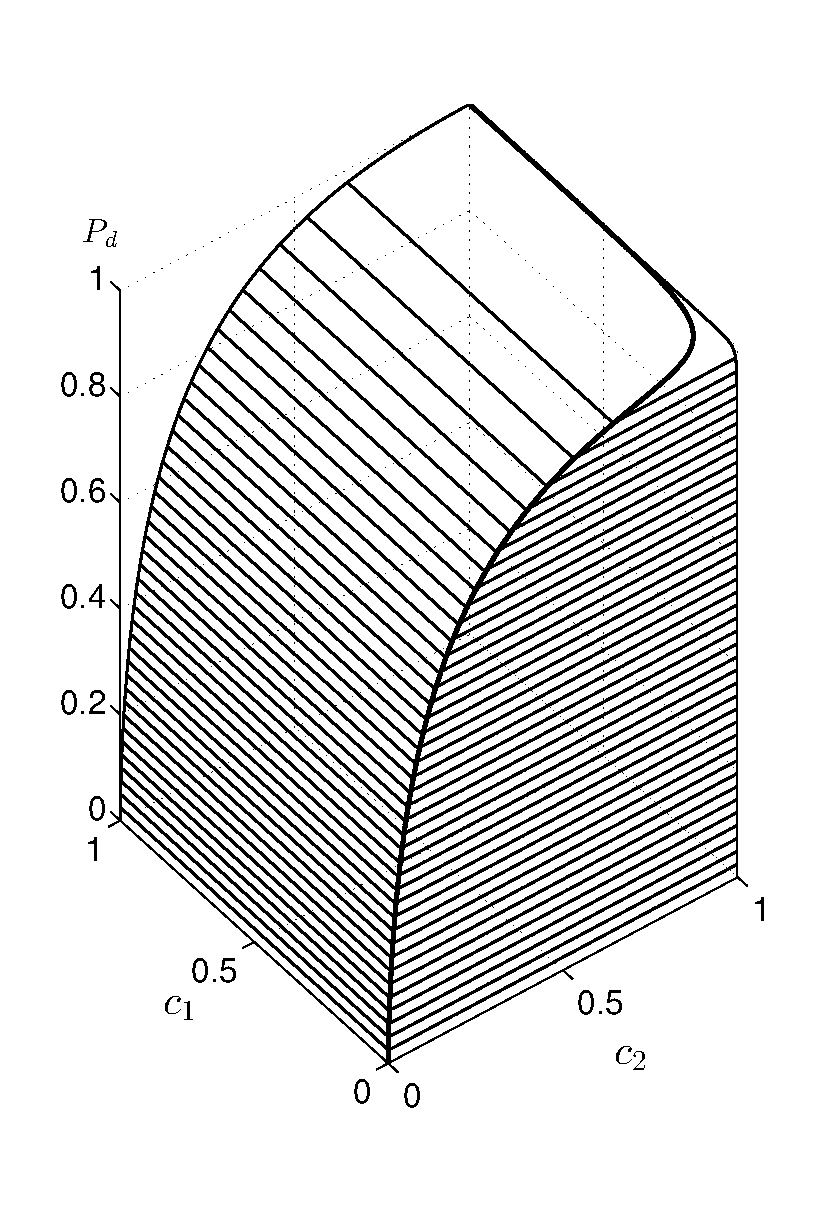
\includegraphics[width=12cm, height=16cm]{3/example3.eps}
\caption{The M-ROC for the Chi-square example.}
\label{pic: LJS for chisquare}
\end{figure}
